\section{Experiment Protocol}

\textbf{Project Title} \\
Evaluation of electrotactile feedback schemes in combination with myoelectric prosthetic control - closing the loop. 

\textbf{Information on Investigators} \\
The investigators are biomedical engineering Master students at Aalborg University. 

\textbf{Background} \\
Losing an upper limb can be hugely debilitating and can result in lowered quality of life due to restrictions in function, appearance and sensation. As a mean to regain the functionality, transradial amputees can receive a functional prosthesis, where the majority are controlled by muscles signals, or myoelectric (EMG) signals. However, still 25\% of myoelectric prosthesis users reject their device, where a major reason for the low satisfaction is due to lack of sensory feedback.
Many advancements have been made in the academic community to improve function accuracy. However, combining function with sensory feedback, thus closing the motor/sensory loop, is still a scarcely investigated area. Therefore, this experiment will combine the control of a prosthesis with sensory feedback delivered via electrotactile stimulation electrodes placed on the forearm. During the experiment the subjects will test two different feedback configurations while controlling a virtual prosthesis, represented as a cursor on a computer screen. The subject can move the cursor in a two-dimensional coordinate system, where the axes represents a degree of freedom (DOF) each (wrist rotation and opened/closed hand).

\textbf{Purpose} \\
The purpose of the experiment is to compare how subjects' perform in an evaluation test when receiving feedback from two different electrotactile stimulation configurations, respectively, in a closed loop virtual prosthesis. This might provide information on which feedback that seems more intuitive to use in practice in a prosthesis.

\textbf{Research Aim} \\
Test and evaluate two novel stimulation schemes, one based on modulating amplitude and one based on spatial localization of activation, for conveying sensory feedback of the prosthesis state in a closed loop prosthetic control system.

\textbf{Experiment Duration} \\
To be estimated.

\textbf{Inclusion Criteria} \\
The subject must be:
\vspace{-15pt}
\begin{itemize}
	\item able bodied. % or transradially amputated as the highest degree of upper limb amputation.
	\item at least 18 years of age.
	\item able to understand, read and speak English and/or Danish.
	\item assessed by the investigators to comply with the instructions given during the experiment.
\end{itemize}

\textbf{Exclusion Criteria} \\
The subject must:
\vspace{-15pt}
\begin{itemize}
	\item not have any diseases/conditions that may influence sensory perception.
	\item be willing to receive low amplitude current stimulation. 
	\item assessed by the investigators to have robust prosthetic control during the experiment.
\end{itemize}

\textbf{{\Large Experiment Description}} \\
\newline
The main aim of the experiment is for the subject to be able to correctly interpret the two sensory feedback schemes when combined with myoelectric prosthetic control. The grid illustrated in \figref{fig:gridmap} is the map the subject will be able to navigate inside. Each square in the map will deliver a different stimulus corresponding to the motion state of the virtual prosthesis, represented as the black cursor. The square with center in the origin (square with cursor inside in \figref{fig:gridmap}) corresponds to resting state and will provide no sensory feedback. The remaining squares in the first row will deliver stimuli corresponding to only the wrist rotation degree of freedom, and the remaining squares in the third column will deliver stimuli only corresponding to the closed hand DOF. The remaining squares will deliver a stimulation based on a combination of the two DOFs. The further away from resting state a square is, corresponds to the angular degree of the prosthesis state in relation to the performed movement (see \figref{fig:sensconfigs}). \\
The arrows in the upper right corner of \figref{fig:gridmap} represent the hand movements needed to be performed to move the cursor in the corresponding direction. The control system will only respond to single DOF movements. Thus, the cursor is only able to move along one axis at a time and not diagonally. The subject will control the cursor with the dominant arm through an EMG electrode armband. The subject will receive stimulation from an electrode consisting of 16 electrode pads placed around the contra-lateral forearm (see illustration in \figref{fig:sensconfigs}).

\begin{figure}
	\subfigure[Illustration of the spatial scheme.]
		{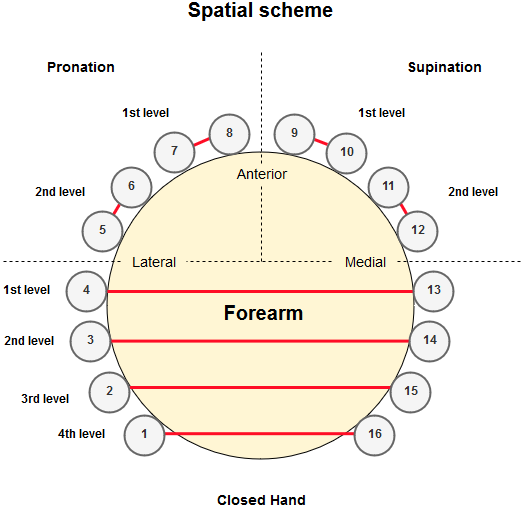
\includegraphics[width=0.48\textwidth]{figures/El_array_spatial}}
	\subfigure[Illustration of the amplitude scheme.]
		{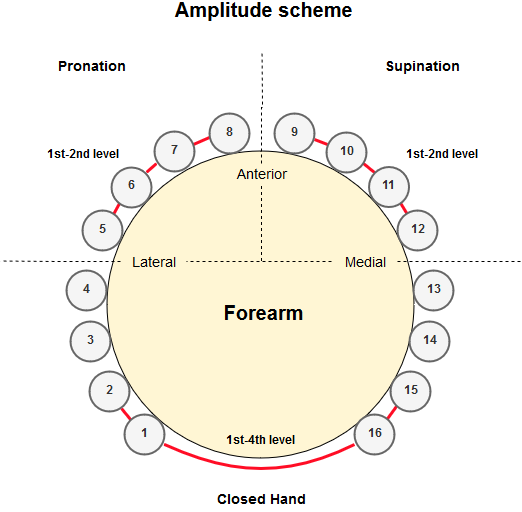
\includegraphics[width=0.48\textwidth]{figures/El_array_amplitude}}
	\caption{Figure (a) shows the spatial scheme, which is based on different electrodes being activated depending on the level of the grid square the cursor is located in. The highest number of possibly activated electrodes is four at a time. Figure (b) shows the amplitude scheme. Here, the amplitude of the active electrodes will increase with the increase of the level of the target location. The highest number of possibly activated electrodes is eight at a time.}
	\label{fig:sensconfigs}
\end{figure}

\begin{figure}[H]                 
	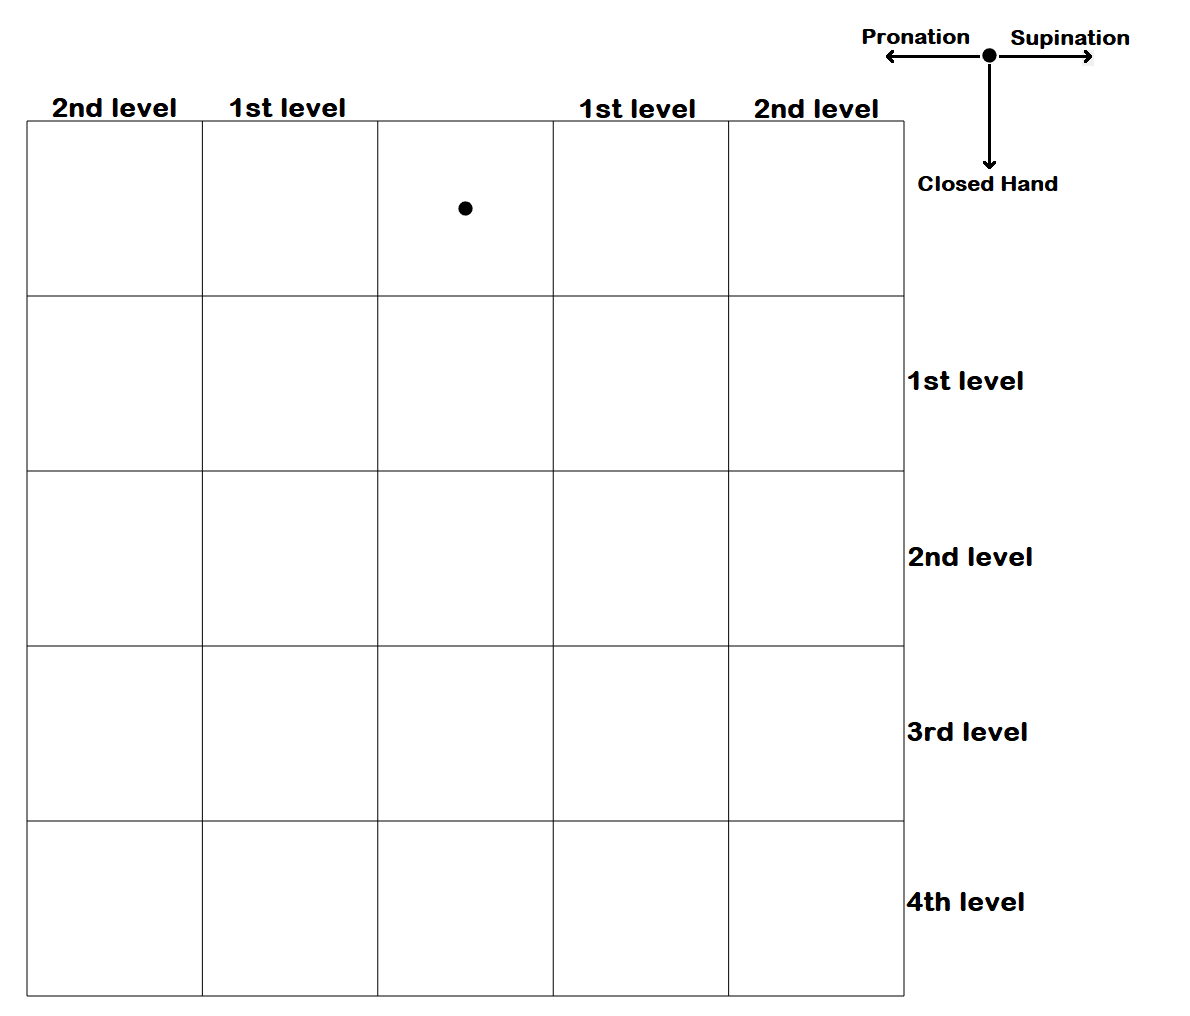
\includegraphics[width=0.9\textwidth]{figures/gridmap2}  
	\caption{Image of the grid map and cursor used in the experiment. Performing supination moves the cursor the right, pronation moves it to the left and closing the hand moves it down. Opening the hand moves the cursor up, and is used as a correction movement if a wrong movement has been made.}
	\label{fig:gridmap} 
\end{figure}


\textbf{{\Large Hand Movements Used for Prosthetic Control}} \\

\begin{figure}[H]                 
	\includegraphics[width=0.6\textwidth]{figures/handmovements}
	\caption{Image of the hand movements used in the experiment for myoelectric prosthetic control. From top left corner: Wrist pronation, wrist supination, opened hand and closed hand.}
	\label{fig:handmovements} 
\end{figure}

\textbf{{\Large Experiment Procedure}} \\
\newline
Before the final evaluation test is carried out the subject will be trained in controlling the cursor via EMG signals, trained in interpreting the sensory feedback and trained in interpreting the sensory feedback while controlling the cursor. The evaluation test is a target reaching test, where the subject needs to move the cursor to a highlighted target consisting of one of the grid squares. The cursor will not be visible, thus, the subject will have to only rely on the information received from the sensory feedback. \\
During the experiment the subject must let the dominant arm hang relaxed down the side of the torso and the contra-lateral arm placed on a table without putting pressure on the stimulation electrode, as seen in \figref{fig:setup}. The subject must be seated during all procedures. The following order represent the chronology of the procedures the subject needs to undergo; the steps will be divided in solely control, solely sensory feedback and feedback with control. 


\textbf{{Control}} \\
\vspace{-25pt}
\begin{enumerate}
	\item Record EMG signals needed to build the prosthetic control system. To do this the subject must first perform  five movements used as reference signals: 15 seconds rest, 15 seconds maximum voluntary contraction (MVC) of wrist supination, 15 seconds MVC of wrist pronation, 15 seconds MVC of opened hand and 15 seconds MVC of closed hand. Between each contraction the subject will get a 15 seconds break to avoid fatigue. Secondly, the subject must perform movements from which the recorded signals are used to build the control system. Here, the subject controls a cursor as seen in \figref{fig:trapezoid}, and must match the cursor with trapezoidal trajectory. The cursor moves horizontally with time and the subject control the contraction intensity vertically. The subject must perform three contractions per movement: 40 \%, 50 \% and 70 \% of the MVC. The plateau of the trapezoidal trajectory corresponds to the designated fraction. Between each performed movement, the subject gets a 15 seconds break to avoid fatigue. Lastly, a 15 seconds rest is recorded. 
	\item Train the subject's ability to control the cursor via letting the subject move freely around inside the grid map for three minutes.
	\item Perform target reaching test to evaluate the subject's ability to control the cursor. The designated target will be one of the squares in the grid highlighted in red. To reach a target the cursor must enter the target and dwell inside it for 1.5 seconds. Then a bell sound will occur and a new target appears. The time limit for reaching a target is 30 seconds. The starting point is always the resting state square (first square in third column), and the cursor will, thus, return to starting point when a target is reached or then the time limit is reached. A total of 16 targets will appear before this test is through.
\end{enumerate}

\begin{figure}[H]                 
	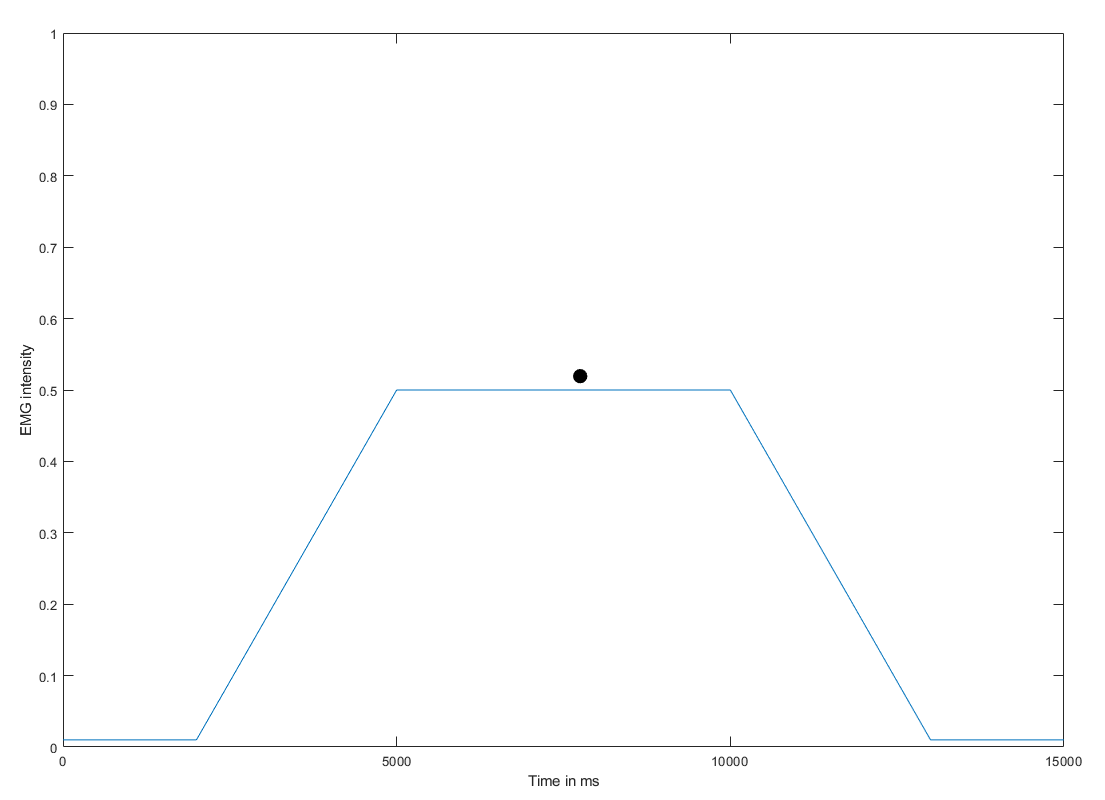
\includegraphics[width=0.65\textwidth]{figures/trapezoid2}  
	\caption{Image of the trapezoidal trajectory used when recording EMG signal used to build the control system. The subject controls the black cursor in height by increasing contraction intensity.}
	\label{fig:trapezoid} 
\end{figure}

\textbf{Sensory Feedback} \\
\vspace{-25pt}
\begin{enumerate}
	\item Record current amplitude thresholds needed to build the sensory feedback schemes. For each electrode the subject must first note when the stimulus with certainty is felt. When all thresholds are set, the sensation of neighbouring electrodes are compared to ensure homogeneity in the sensation. Afterwards the same procedure is performed for the subject's tolerance threshold. 
	\item Train the subject's ability to interpret sensory feedback of feedback one of the schemes. This is done  by exposing the subject to feedback from all grid squares. The subject will experience the transitions from square to square until the designated square is reached.  
	\item Perform reinforcement learning on 16 grid different squares. During this step the subject will be turned away from the computer screen. When a designated square is reached, the subject will be asked where the cursor is located. After answering the subject will be informed on whether is was correct, and told the correct location, if the answer was incorrect. 
	\item Perform validation test on the 16 squares from step 3. The order of the squares and the route to each square will vary from step 3. During this step the subject must look away from the computer screen. When a designated square is reached, the subject will be asked where the cursor is located. After answering the subject will not be informed whether the answer was correct or not.
\end{enumerate}

\textbf{Sensory Feedback with Control} \\
\vspace{-25pt}
\begin{enumerate}
	\item Train the subject's ability to control the cursor while receiving sensory feedback via letting the subject move freely around inside the grid map for three minutes.
	\item Perform target reaching test where the cursor is invisible to evaluate how well the subject can utilize the sensory feedback regarding the cursor location. This test has the same format as the target reaching test from the control procedure step 3.
	\item Redo sensory feedback steps and sensory feedback with control steps with sensory feedback from the remaining scheme.
\end{enumerate}


\newpage
\textbf{{\Large Experiment Setup}} \\

\begin{figure}[H]                 
	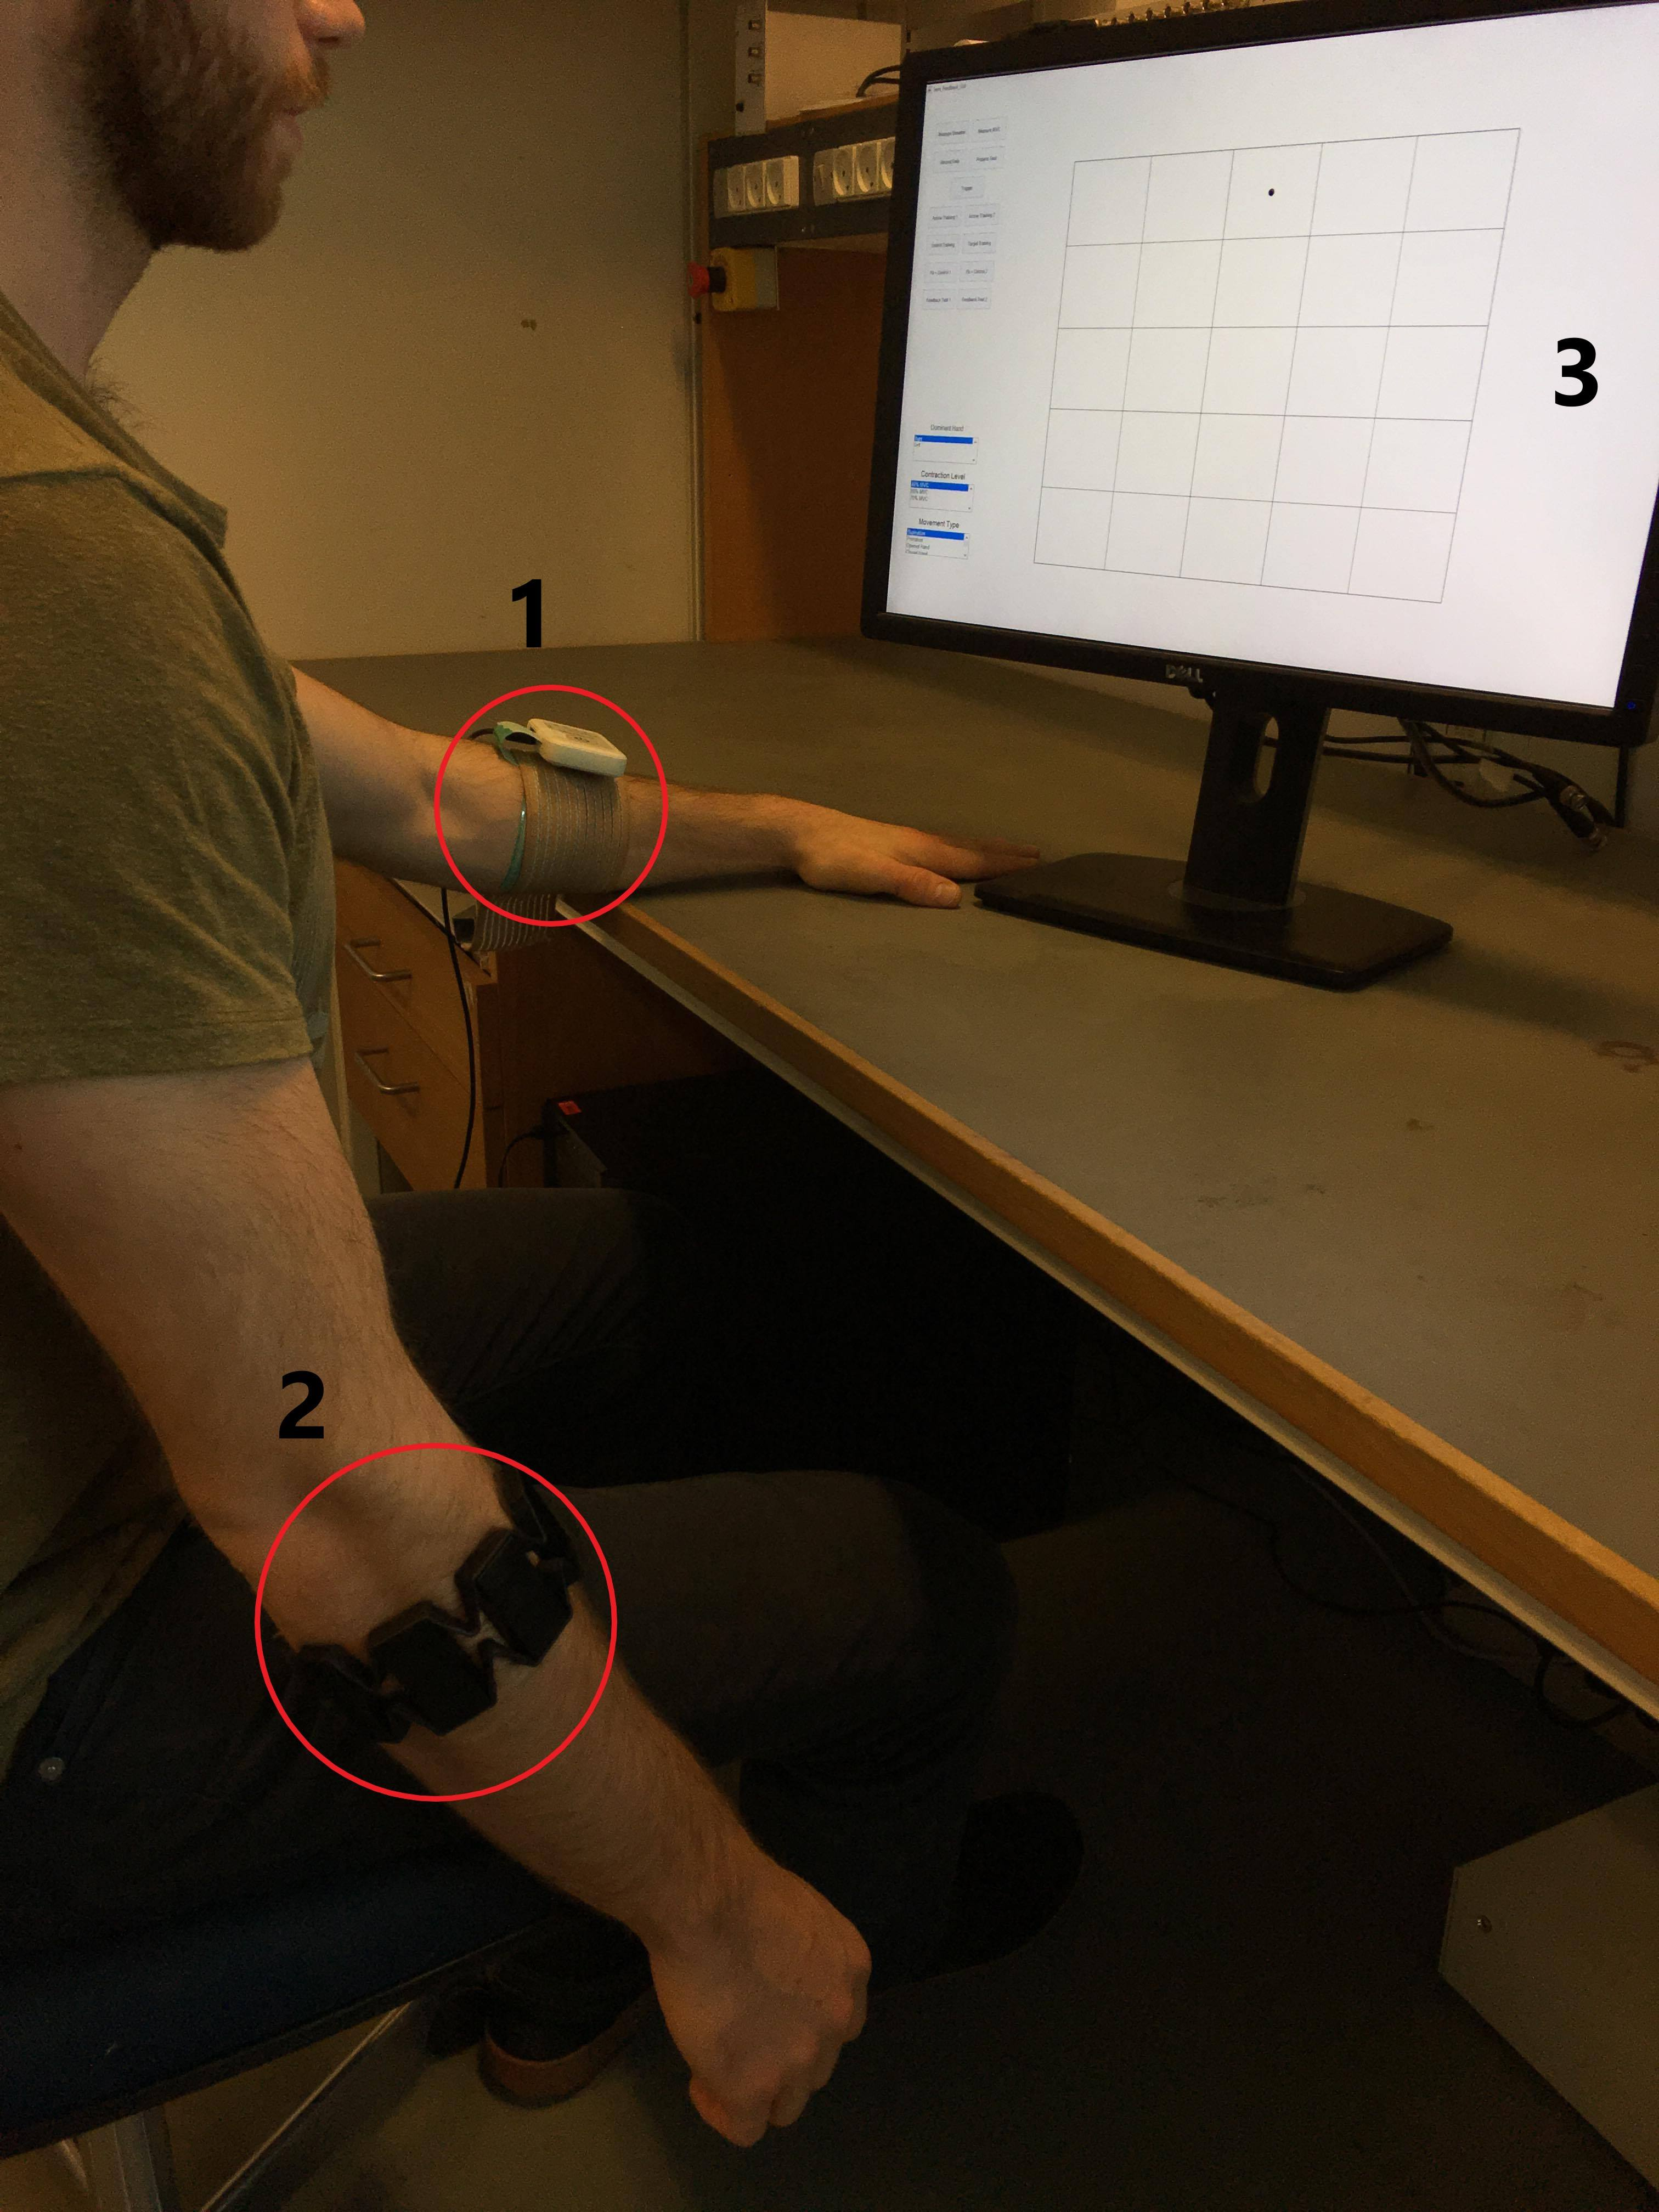
\includegraphics[width=0.8\textwidth]{figures/setupimg}  
	\caption{Image of the experimental setup. 1) is the stimulation device with the stimulation electrode placed under the brown armband, 2) is the electrode armband used to record EMG signals and 3) is the computer screen used to guide the subject and display tasks.} 
	\label{fig:setup} 
\end{figure}

